\documentclass[11pt]{article}

% Language setting
\usepackage[turkish]{babel}
\usepackage{pythonhighlight}

\usepackage[a4paper,top=2cm,bottom=2cm,left=2cm,right=2cm,marginparwidth=2cm]{geometry}

% Useful packages
\usepackage{amsmath}
\usepackage{graphicx}
\usepackage[colorlinks=true, allcolors=blue]{hyperref}
\usepackage{verbatim}
\usepackage{fancyhdr} % for header and footer
\usepackage{titlesec}
\usepackage{parskip}

\setlength{\parindent}{0pt}

\titleformat{\subsection}[runin]{\bfseries}{\thesubsection}{1em}{}

\pagestyle{fancy} % activate the custom header/footer

% define the header/footer contents
\lhead{\small{23BLM-4014 Yapay Sinir Ağları Ara Sınav Soru ve Cevap Kağıdı}}
\rhead{\small{Dr. Ulya Bayram}}
\lfoot{}
\rfoot{}

% remove header/footer on first page
\fancypagestyle{firstpage}{
  \lhead{}
  \rhead{}
  \lfoot{}
  \rfoot{\thepage}
}
 

\title{Çanakkale Onsekiz Mart Üniversitesi, Mühendislik Fakültesi, Bilgisayar Mühendisliği Akademik Dönem 2022-2023\\
Ders: BLM-4014 Yapay Sinir Ağları/Bahar Dönemi\\ 
ARA SINAV SORU VE CEVAP KAĞIDI\\
Dersi Veren Öğretim Elemanı: Dr. Öğretim Üyesi Ulya Bayram}
\author{%
\begin{minipage}{\textwidth}
\raggedright
Öğrenci Adı Soyadı: ÖZNUR KAN\\ % Adınızı soyadınızı ve öğrenci numaranızı noktaların yerine yazın
Öğrenci No: 180401046
\end{minipage}%
}

\date{14 Nisan 2023}

\begin{document}
\maketitle

\vspace{-.5in}
\section*{Açıklamalar:}
\begin{itemize}
    \item Vizeyi çözüp, üzerinde aynı sorular, sizin cevaplar ve sonuçlar olan versiyonunu bu formatta PDF olarak, Teams üzerinden açtığım assignment kısmına yüklemeniz gerekiyor. Bu bahsi geçen PDF'i oluşturmak için LaTeX kullandıysanız, tex dosyasının da yer aldığı Github linkini de ödevin en başına (aşağı url olarak) eklerseniz bonus 5 Puan! (Tavsiye: Overleaf)
    \item Çözümlerde ya da çözümlerin kontrolünü yapmada internetten faydalanmak, ChatGPT gibi servisleri kullanmak serbest. Fakat, herkesin çözümü kendi emeğinden oluşmak zorunda. Çözümlerinizi, cevaplarınızı aşağıda belirttiğim tarih ve saate kadar kimseyle paylaşmayınız. 
    \item Kopyayı önlemek için Github repository'lerinizin hiçbirini \textbf{14 Nisan 2023, saat 15:00'a kadar halka açık (public) yapmayınız!} (Assignment son yükleme saati 13:00 ama internet bağlantısı sorunları olabilir diye en fazla ekstra 2 saat daha vaktiniz var. \textbf{Fakat 13:00 - 15:00 arası yüklemelerden -5 puan!}
    \item Ek puan almak için sağlayacağınız tüm Github repository'lerini \textbf{en geç 15 Nisan 2023 15:00'da halka açık (public) yapmış olun linklerden puan alabilmek için!}
    \item \textbf{14 Nisan 2023, saat 15:00'dan sonra gönderilen vizeler değerlendirilmeye alınmayacak, vize notu olarak 0 (sıfır) verilecektir!} Son anda internet bağlantısı gibi sebeplerden sıfır almayı önlemek için assignment kısmından ara ara çözümlerinizi yükleyebilirsiniz yedekleme için. Verilen son tarih/saatte (14 Nisan 2023, saat 15:00) sistemdeki en son yüklü PDF geçerli olacak.
    \item Çözümlerin ve kodların size ait ve özgün olup olmadığını kontrol eden bir algoritma kullanılacaktır. Kopya çektiği belirlenen vizeler otomatikman 0 (sıfır) alacaktır. Bu nedenle çözümlerinizi ve kodlarınızı yukarıda sağladığım gün ve saatlere kadar kimseyle paylaşmayınız.
    \item Bu vizeden alınabilecek en yüksek not 100'dür. Toplam aldığınız puan 100'ü geçerse, aldığınız not 100'e sabitlenecektir.
    \item LaTeX kullanarak PDF oluşturanlar öz geçmişlerine LaTeX bildiklerini de eklemeyi unutmasınlar :)
    \item Bu vizedeki soruların çözümleri ve tex dosyası için istediğiniz kadar sayıda Github repository'si oluşturabilirsiniz. Sadece yukarıda belirttiğim tarihlerde (14 Nisan 2023 saat 15:00 ile 15 Nisan 2023 saat 15:00 arasında) public yapmayı/halka açmayı ve Github profilinizi de öz geçmişinize eklemeyi unutmayın :)
    \item Bilgisayarınıza hiçbir program kurmadan, Overleaf, Google Colab, Kaggle gibi ortamlar üzerinden bu vizeyi tamamlamanız mümkün. İyi çalışmalar!!
\end{itemize}

(Ekstra 5 puan) \url{https://github.com/oznurkan/Project_artificial_neural_network_tex/upload/main}

\newpage
\section{(Toplam 10 Puan) Hopfield Networks:}

\subsection{(2 Puan)} \textbf{ChatGPT’ye size Hopfield Network’ler ile ilgili detaylı bilgi vermesini isteyin. Sorduğunuz soruyu, ChatGPT'nin çıkartığı cevabı aşağı koyun. Bu cevapta anlamadığınız terimleri de ChatGPT’ye sorup, sorduğunuz soruları ve ChatGPT’nin verdiği cevapları da sırayla aşağı koyun.}

\textbf{SORU (CHATGPT) =} Hopfield Network’ler ile ilgili detaylı bilgi verebilir misin?

\textbf{CEVAP =} Hopfield ağları, sinir ağı modellerinden biridir ve en eski ve popüler olanlarından biridir. Hopfield ağları, birbiriyle etkileşim halinde olan bir dizi nöron (veya hücre) koleksiyonudur. Her nöron, girdi olarak diğer nöronların çıkışını alır ve çıkışı da diğer nöronların girdisine eklenir. Böylece, her nöron, diğer nöronların aktivasyonu ile belirlenir.

Hopfield ağları, özellikle bellek veya tanıma sorunları için kullanılır. Ağ, bir bellek çiftini depolayabilir ve ardından bir girdi verildiğinde, depolanmış belleklerden birini hatırlamaya çalışır. Hopfield ağları, asenkron dinamikleri ile çalışır, yani tüm nöronlar eşzamanlı olarak değil, sırayla güncellenir.

Bir Hopfield ağı, genellikle iki durumlu (on-off) nöronlar kullanır. Her nöron, iki durumlu bir cihaz gibi davranır ve bu durumlar, genellikle 1 ve -1 olarak tanımlanan birçok farklı şekilde belirlenebilir. Ayrıca ağ, bir enerji fonksiyonu kullanır, böylece ağın durumunu bir enerji seviyesiyle ifade edebilirsiniz.

Hopfield ağları, birçok farklı uygulamada kullanılabilir. Örneğin, bunlar veri sıkıştırma, modelleme ve tanıma, ham verilerin temizlenmesi ve hatırlama sorunları gibi alanlarda kullanılabilir.

Hopfield ağlarının bir dezavantajı, büyük ölçekli problemlerde çalışırken verimliliklerinin azalmasıdır. Bu nedenle, daha büyük ölçekli problemlerde, özellikle daha karmaşık sinir ağı modelleri kullanmak daha verimlidir.


\subsection{(8 Puan)} \textbf{ChatGPT’nin açıklamalarından ne anladığınızı buraya kendi kelimelerinizle özetleyin. Örneğin ``Hopfield Network nedir? Ne işe yarar? Neden bilmemiz gerekir bunu? Gerçek hayatta kullanılıyor mu?'' gibi. Anlamadığınız kısımlar varsa ve ChatGPT’nin açıklamaları yeterli gelmezse internet dahil farklı kaynaklardan araştırıp, bilgilerin doğruluğunu sorgulamakta serbestsiniz. Konuyu doğru anlayıp anlamamanız puana etki edecektir. Kullandığınız kaynakları da belirtin!}

\textbf{SORU (CHATGPT ) =} Hopfield Network nedir? 

\textbf{CEVAP (CHATGPT and me) =} Hopfield ağı, bir tür sinir ağı modelidir. Birbirine bağlı bir dizi nöron koleksiyonundan oluşur ve bellek veya tanıma sorunları için kullanılır. Ağ, bir bellek çiftini depolayabilir ve ardından bir girdi verildiğinde, depolanmış belleklerden birini hatırlamaya çalışır. Hopfield ağları, asenkron dinamikleri ile çalışır. Hopfield ağları biyolojik sinir ağlarının matematiksel modellemesi için de kullanılabilir.

\textbf{SORU (CHATGPT) =} Ne işe yarar? 

\textbf{CEVAP =} Hopfield ağları, bellek veya tanıma sorunlarının çözülmesinde kullanılır. Ağ, bir bellek çiftini depolayabilir ve ardından bir girdi verildiğinde, depolanmış belleklerden birini hatırlamaya çalışır. Özellikle veri sıkıştırma, modelleme ve tanıma, ham verilerin temizlenmesi ve hatırlama sorunları gibi alanlarda kullanılır. Hopfield ağları, ayrıca biyolojik sinir ağlarının matematiksel modellemesi için de kullanılabilir. Bunun yanı sıra, sınırlı bellekli ve düşük güç tüketimli çip tasarımlarında da sık kullanılır.

\textbf{SORU (CHATGPT) =} Neden bilmemiz gerekir bunu? 

\textbf{CEVAP =} Hopfield ağlarının ne olduğunu ve nasıl çalıştığını bilmek, yapay zeka ve sinir ağı modelleri hakkında bilgi sahibi olmak isteyen kişiler için önemlidir. Bu ağlar, bellek veya tanıma sorunlarının çözümü için kullanılan güçlü bir araçtır ve birçok alanda kullanım potansiyeli vardır. Ayrıca, Hopfield ağları biyolojik sinir ağlarının matematiksel modellemesi için kullanılabileceğinden, nörobilim araştırmalarında da kullanılmaktadır. Dolayısıyla, Hopfield ağlarını bilmek, yapay zeka, sinir ağı modelleri, bellek veya tanıma sorunları, cihaz tasarımı ve nörobilim gibi konularda ilgi duyanlar için faydalı olabilir.

\textbf{SORU (CHATGPT) =} Gerçek hayatta kullanılıyor mu?

\textbf{CEVAP =} Evet, Hopfield ağları gerçek hayatta birçok alanda kullanılmaktadır. Örneğin, Hopfield ağları, veri sıkıştırma, modelleme ve tanıma, ham verilerin temizlenmesi ve hatırlama sorunları gibi alanlarda kullanılır. Hopfield ağları ayrıca, sınırlı bellekli ve düşük güç tüketimli çip tasarımlarında da sık kullanılır. Bunun yanı sıra, Hopfield ağları biyolojik sinir ağlarının matematiksel modellemesi için kullanılabileceğinden, nörobilim araştırmalarında da kullanılmaktadır. Dolayısıyla, Hopfield ağları, gerçek hayatta yaygın bir şekilde kullanılan bir yapay sinir ağı modelidir.


\section{(Toplam 10 Puan) Boltzman Machine:}

\subsection{(2 Puan)} \textbf{ChatGPT’ye size Boltzman Machine ilgili detaylı bilgi vermesini isteyin. Sorduğunuz soruyu, ChatGPT'nin çıkartığı cevabı aşağı koyun. Bu cevapta anlamadığınız terimleri de ChatGPT’ye sorup, sorduğunuz soruları ve ChatGPT’nin verdiği cevapları da sırayla aşağı koyun.}

\textbf{SORU (CHATGPT) =} Boltzman Machine ilgili detaylı bilgi verebilir misin?

\textbf{CEVAP =} Boltzmann Machine (BM), yapay sinir ağı modellerinden biridir ve özellikle büyük ve karmaşık veri kümelerini analiz etmek için kullanılır. Adını istatistik mekaniğin önemli isimlerinden olan Ludwig Boltzmann'dan almıştır. Boltzmann Machine, özellikle desen tanıma, doğal dil işleme, nesne tanıma, sınıflandırma ve öneri sistemleri gibi alanlarda kullanılır.

BM, iki tip nöronun birbiriyle etkileşimini içerir: Görünür ve Gizli nöronlar. Görünür nöronlar, veri kümesinde doğrudan gözlemlenebilen nöronlardır. Gizli nöronlar ise, sadece diğer gizli nöronlar ve görünür nöronlarla etkileşimde bulunarak veri üzerindeki gizli yapıları belirleyebilirler.

BM, verilerin enerji seviyelerinin azaltıldığı bir süreç olan eğitim sürecinde öğrenir. BM, bir matematiksel enerji fonksiyonu kullanarak çalışır. Bu fonksiyon, bir veri örneği için bir enerji değeri hesaplar ve bu enerji değeri, verinin ne kadar "iyi" veya "kötü" olduğunu temsil eder.

BM, eğitim sırasında bir öğrenme algoritması kullanarak veri kümesini işler ve ağırlıklarını, enerji fonksiyonunu minimize edecek şekilde ayarlar. Bir kez eğitildikten sonra, BM, belirli bir girdiye yanıt vermek üzere kullanılabilir.

BM, özellikle büyük ve karmaşık veri kümeleri üzerinde çalışırken, veri içindeki desenleri keşfetmek için kullanılır. Örneğin, bir BM, bir görüntüdeki nesneleri tanımak, bir doğal dil belgesindeki kelimeleri tanımak veya bir müşterinin alışveriş alışkanlıklarını öğrenmek için kullanılabilir.

BM, derin öğrenme alanında önemli bir konudur ve birçok farklı türü vardır. Bunlar arasında Sınır İtici Boltzmann Makinesi (RBM), Tersinir Boltzmann Makinesi (DBN) ve Etkileşimli Boltzmann Makinesi (IBM) bulunur.

Sonuç olarak, Boltzmann Machine, yapay zeka ve makine öğrenimi gibi teknolojilerde önemli bir rol oynar ve büyük veri kümelerinin analizi için çok faydalıdır. Bu teknolojinin anlaşılabilecek şekilde açıklanması, insanların bu alanda çalışan araştırmacıların geliştirdiği yenilikleri anlamasına yardımcı olur.

\subsection{(8 Puan)} \textbf{ChatGPT’nin açıklamalarından ne anladığınızı buraya kendi kelimelerinizle özetleyin. Örneğin ``Boltzman Machine nedir? Ne işe yarar? Neden bilmemiz gerekir bunu? Gerçek hayatta kullanılıyor mu?'' gibi. Anlamadığınız kısımlar varsa ve ChatGPT’nin açıklamaları yeterli gelmezse internet dahil farklı kaynaklardan araştırıp, bilgilerin doğruluğunu sorgulamakta serbestsiniz. Konuyu doğru anlayıp anlamamanız puana etki edecektir. Kullandığınız kaynakları da belirtin!}

\textbf{SORU (CHATGPT) =} Boltzman Machine nedir?

\textbf{CEVAP =} Boltzmann Machine (BM) iki tip nöronun birbiriyle etkileşimini içeren yapay sinir ağı modellerinden biridir ve özellikle büyük ve karmaşık veri kümelerini analiz etmek için kullanılır.Bu iki tip Görünür ve Gizli nöronlardır. Görünür nöronlar, veri kümesinde doğrudan gözlemlenebilen nöronlardır. Gizli nöronlar ise, sadece diğer gizli nöronlar ve görünür nöronlarla etkileşimde bulunarak veri üzerindeki gizli yapıları belirleyebilirler.

 BM, bir matematiksel enerji fonksiyonu kullanarak çalışır. Bu fonksiyon, bir veri örneği için bir enerji değeri hesaplar ve bu enerji değeri, verinin ne kadar "iyi" veya "kötü" olduğunu temsil eder.
 
 BM, eğitim sırasında bir öğrenme algoritması kullanarak veri kümesini işler ve ağırlıklarını, enerji fonksiyonunu minimize edecek şekilde ayarlar. Bir kez eğitildikten sonra, BM, belirli bir girdiye yanıt vermek üzere kullanılabilir.

BM, özellikle büyük ve karmaşık veri kümeleri üzerinde çalışırken, veri içindeki desenleri keşfetmek için kullanılır. Örneğin, bir BM, bir görüntüdeki nesneleri tanımak, bir doğal dil belgesindeki kelimeleri tanımak veya bir müşterinin alışveriş alışkanlıklarını öğrenmek için kullanılabilir.

\textbf{SORU (CHATGPT) =} Ne işe yarar?

\textbf{CEVAP =} Boltzmann Machine (BM), büyük ve karmaşık veri kümelerini analiz etmek için kullanılır. BM, veri içindeki desenleri keşfetmek için kullanılır.Bir görüntüdeki nesneleri tanımak, bir doğal dil belgesindeki kelimeleri tanımak veya bir müşterinin alışveriş alışkanlıklarını öğrenmek için kullanılabilir.

BM, özellikle derin öğrenme alanında önemli bir konudur. BM'nin farklı türleri, örneğin Sınır İtici Boltzmann Makinesi (RBM), Tersinir Boltzmann Makinesi (DBN) ve Etkileşimli Boltzmann Makinesi (IBM) gibi, farklı problemler için özelleştirilebilir ve uyarlanabilir.

BM, özellikle veri analizi, doğal dil işleme, görüntü işleme ve öneri sistemleri gibi alanlarda kullanılır. BM, bu alanlarda birçok uygulama bulabilir, örneğin bir müşterinin alışveriş alışkanlıklarına dayalı olarak öneriler sunmak, bir görüntüdeki nesneleri tanımak veya bir metin belgesindeki anahtar kelimeleri belirlemek gibi.

BM, özellikle büyük veri kümeleri için kullanışlıdır ve geleneksel makine öğrenme teknikleri bu verileri işlemekte yetersiz kalabilir. BM, veri içindeki yapıları keşfetmek için kullanılabildiği için, yeni fikirlerin ve ilişkilerin keşfi için de kullanılabilir.

\textbf{SORU (CHATGPT) =} Neden bilmemiz gerekir bunu?

\textbf{CEVAP =} Boltzmann Machine (BM), derin öğrenme alanında önemli bir konudur ve büyük veri kümelerini analiz etmek için kullanılır. Günümüzde, birçok farklı endüstri, özellikle veri analizi, doğal dil işleme, görüntü işleme ve öneri sistemleri gibi alanlarda BM teknolojilerini kullanmaktadır.

Bu nedenle, BM teknolojileri hakkında bilgi sahibi olmak, günümüzdeki birçok endüstrinin veri analizi süreçlerinde faydalıdır. BM, büyük veri kümeleri üzerinde çalışırken, veri içindeki desenleri keşfetmek için kullanılır ve bu da farklı problemleri çözmek için kullanılabilir.

Ayrıca, BM teknolojilerinin işleyişinin anlaşılması, derin öğrenme alanında çalışan araştırmacılar ve geliştiriciler için de önemlidir. BM, özellikle büyük ve karmaşık veri kümeleri üzerinde çalışırken, diğer makine öğrenme tekniklerinden farklı bir yaklaşım sunar ve bu nedenle, öğrenme süreci ve veri analizi süreci için farklı bir bakış açısı sağlar.

Sonuç olarak, BM hakkında bilgi sahibi olmak, günümüzdeki veri analizi süreçlerinde daha verimli ve etkili bir şekilde çalışmak için faydalıdır ve derin öğrenme alanında çalışanlar için de önemlidir.

\textbf{SORU (CHATGPT) =} Gerçek hayatta kullanılıyor mu?

\textbf{CEVAP =} Evet, Boltzmann Machine (BM) gerçek hayatta birçok alanda kullanılıyor. Özellikle, büyük veri kümelerinin analizi için kullanılan BM teknolojileri, birçok endüstride yaygın olarak kullanılıyor.

BM, özellikle veri analizi, doğal dil işleme, görüntü işleme ve öneri sistemleri gibi alanlarda kullanılmaktadır. Örneğin, bir online mağaza, müşteri davranışlarını analiz etmek ve müşterilere öneriler sunmak için BM teknolojilerini kullanabilir. Benzer şekilde, bir arama motoru, arama sonuçlarını belirlemek için BM kullanabilir ve bir görüntü tanıma sistemleri, görüntülerdeki nesneleri tanımak için BM teknolojilerinden faydalanabilir.

BM ayrıca, derin öğrenme alanında önemli bir konudur ve birçok farklı uygulama ve teknolojiyi de içeren geniş bir araştırma alanıdır. Örneğin, Sınır İtici Boltzmann Makineleri (RBM), Tersinir Boltzmann Makineleri (DBN) ve Etkileşimli Boltzmann Makineleri (IBM) gibi farklı BM türleri, farklı problemler için özelleştirilebilir ve uyarlanabilir.

Sonuç olarak, BM teknolojileri, gerçek hayatta birçok farklı alanda kullanılmaktadır ve büyük veri kümelerinin analizi için son derece önemlidir. Ayrıca, derin öğrenme alanında araştırma yapmak için de önemli bir konudur.

\section{(Toplam 10 Puan) Markov Assumption ve Markov Chain:}

\subsection{(2 Puan)} \textbf{ChatGPT’ye size Markov assumption ve Markov Chain ilgili detaylı bilgi vermesini isteyin. Sorduğunuz soruyu, ChatGPT'nin çıkartığı cevabı aşağı koyun. Bu cevapta anlamadığınız terimleri de ChatGPT’ye sorup, sorduğunuz soruları ve ChatGPT’nin verdiği cevapları da sırayla aşağı koyun.}

\textbf{SORU (CHATGPT) =} Markov assumption ve Markov Chain ilgili detaylı bilgi verebilir misin?

\textbf{CEVAP =} Markov süreci ya da Markov Zinciri, bir sistemin geçmiş durumları yerine sadece şu anki durumuna bağlı olduğu varsayımıyla modellenir. Bu varsayıma "Markov varsayımı" denir. Bu varsayım, bir sonraki durumun yalnızca şu anki duruma bağlı olduğunu varsayar ve önceki durumların ve geçmiş durumların bilinmesine gerek yoktur.

Markov zinciri, bir dizi adımdan oluşan bir süreçtir. Her adımda, sistem belli bir durumda bulunur ve bir sonraki durum, geçmiş durumlardan bağımsız olarak, olasılıksal bir şekilde belirlenir. Bu olasılıklar, bir geçiş matrisi olarak adlandırılır ve her satır, bir durumu temsil eder ve her sütun, bir sonraki durumu temsil eder.

Markov zincirleri birçok alanda kullanılır, özellikle de doğal dil işleme, finans, biyoloji ve fizikte. Örneğin, dil modelleri, her kelimenin önceki kelimeye bağlı olduğu bir Markov zinciri olarak modellenebilir.

Markov zincirleri, özellikle kuyruklu Markov zincirleri, geleceği tahmin etmek, sınıflandırma yapmak, dönemik sistemleri modellerlemek ve veri sıkıştırmada kullanılır.


\subsection{(8 Puan)} \textbf{ChatGPT’nin açıklamalarından ne anladığınızı buraya kendi kelimelerinizle özetleyin. Örneğin ``Markov assumption ve Markov Chain nedir? Ne işe yarar? Neden bilmemiz gerekir bunu? Gerçek hayatta kullanılıyor mu?'' gibi. Anlamadığınız kısımlar varsa ve ChatGPT’nin açıklamaları yeterli gelmezse internet dahil farklı kaynaklardan araştırıp, bilgilerin doğruluğunu sorgulamakta serbestsiniz. Konuyu doğru anlayıp anlamamanız puana etki edecektir. Kullandığınız kaynakları da belirtin!}

\textbf{SORU (CHATGPT) =} Markov assumption ve Markov Chain nedir?

\textbf{CEVAP =} Markov varsayımı, bir sistemin gelecekteki durumu, sadece o anki durumuna bağlı olduğunu varsayar ve önceki durumların bilinmesine gerek yoktur. Markov zinciri ise, bu varsayıma dayanan ve bir dizi adımdan oluşan bir süreçtir. Her adımda, sistem belirli bir durumda bulunur ve bir sonraki durum, geçmiş durumlardan bağımsız olarak, olasılıksal bir şekilde belirlenir.

Markov zincirleri, birçok alanda kullanılır. Özellikle, doğal dil işleme, finans, biyoloji ve fizikte kullanılır. Dil modelleri, örneğin, her kelimenin önceki kelimeye bağlı olduğu bir Markov zinciri olarak modellenebilir. Bu zincirler, geleceği tahmin etmek, sınıflandırma yapmak, dönemik sistemleri modellerlemek ve veri sıkıştırmada kullanılır.


\textbf{SORU (CHATGPT) =} Ne işe yarar?

\textbf{CEVAP =} Markov zincirleri, sistemin geçmiş durumları yerine sadece şu anki durumuna bağlı olduğu varsayımıyla modellenir. Bu varsayım, bir sonraki durumun yalnızca şu anki duruma bağlı olduğunu varsayar ve önceki durumların ve geçmiş durumların bilinmesine gerek yoktur. Bu nedenle, Markov zincirleri geleceği tahmin etmek, sınıflandırma yapmak, dönemik sistemleri modellerlemek ve veri sıkıştırmada kullanılır.

Örneğin, doğal dil işlemede, bir dil modeli, her kelimenin önceki kelimeye bağlı olduğu bir Markov zinciri olarak modellenebilir. Bu model, bir kelimenin ardından gelen kelimenin olasılığını tahmin etmek için kullanılabilir. Finansal piyasalarda, hisse senedi fiyatları veya döviz kurları için Markov zincirleri kullanılarak gelecekteki fiyatların tahmini yapılabilir. Biyolojide, Markov zincirleri, proteinlerin yapılarının modellenmesi ve moleküler dinamik simülasyonları gibi alanlarda kullanılır.

Markov zincirleri, ayrıca rastgele yürüyüşler ve istatistiksel mekanik gibi fiziksel sistemlerin modellenmesinde de kullanılır.


\textbf{SORU (CHATGPT) =} Neden bilmemiz gerekir bunu?

\textbf{CEVAP =} Markov zincirleri ve Markov varsayımı, birçok alanda kullanılan önemli matematiksel kavramlardır. Bu nedenle, bu konuda bilgi sahibi olmak, birçok alanda çalışan ve bu süreçleri kullanmayı düşünen insanlar için önemlidir. Örneğin, finansal piyasalarda çalışanlar, hisse senedi fiyatlarının tahmini için Markov zincirlerini kullanabilirler. Biyoloji alanında çalışanlar, proteinlerin yapılarının modellenmesi için Markov zincirlerini kullanabilirler. Doğal dil işlemede çalışanlar, dil modelleri oluşturmak için Markov zincirlerini kullanabilirler.

Markov zincirleri ayrıca makine öğrenmesi ve yapay zeka alanlarında da sıkça kullanılır. Bu nedenle, bu konuda bilgi sahibi olmak, gelecekte bu alanda çalışmak isteyenler için de önemlidir.


\textbf{SORU (CHATGPT) =} Gerçek hayatta kullanılıyor mu?

\textbf{CEVAP =} Evet, Markov zincirleri gerçek hayatta birçok alanda kullanılır. Örneğin:

Doğal Dil İşleme: Doğal dil işlemede, dil modelleri oluşturmak için Markov zincirleri kullanılır. Bu modeller, bir kelimenin ardından gelen kelimenin olasılığını tahmin etmek için kullanılır. Örneğin, bir kelime işlemcinin otomatik tamamlama özelliğinde kullanılabilir.

Finans: Finansal piyasalarda, hisse senedi fiyatları veya döviz kurları için Markov zincirleri kullanılarak gelecekteki fiyatların tahmini yapılabilir. Bu tahminler, yatırımcıların piyasayı anlamalarına ve karar vermelerine yardımcı olabilir.

Biyoloji: Biyolojide, proteinlerin yapılarının modellenmesi için Markov zincirleri kullanılır. Bu modeller, proteinlerin yapısını tahmin etmek için kullanılabilir.

Fizik: Markov zincirleri, rastgele yürüyüşler ve istatistiksel mekanik gibi fiziksel sistemlerin modellenmesinde de kullanılır. Bu modeller, moleküler dinamik simülasyonları gibi alanlarda kullanılabilir.

Makine Öğrenmesi: Markov zincirleri, makine öğrenmesi ve yapay zeka alanlarında da sıkça kullanılır. Örneğin, konuşma tanıma ve metin sınıflandırma gibi uygulamalarda kullanılabilir.

Bu örnekler gösteriyor ki, Markov zincirleri gerçek hayatta birçok alanda kullanılan önemli bir matematiksel kavramdır.


\section{(Toplam 20 Puan) Feed Forward:}
 
\begin{itemize}
    \item Forward propagation için, input olarak şu X matrisini verin (tensöre çevirmeyi unutmayın):\\
    $X = \begin{bmatrix}
        1 & 2 & 3\\
        4 & 5 & 6
        \end{bmatrix}$
    Satırlar veriler (sample'lar), kolonlar öznitelikler (feature'lar).
    \item Bir adet hidden layer olsun ve içinde tanh aktivasyon fonksiyonu olsun
    \item Hidden layer'da 50 nöron olsun
    \item Bir adet output layer olsun, tek nöronu olsun ve içinde sigmoid aktivasyon fonksiyonu olsun
\end{itemize}

Tanh fonksiyonu:\\
$f(x) = \frac{exp(x) - exp(-x)}{exp(x) + exp(-x)}$
\vspace{.2in}

Sigmoid fonksiyonu:\\
$f(x) = \frac{1}{1 + exp(-x)}$

\vspace{.2in}
 \textbf{Pytorch kütüphanesi ile, ama kütüphanenin hazır aktivasyon fonksiyonlarını kullanmadan, formülünü verdiğim iki aktivasyon fonksiyonunun kodunu ikinci haftada yaptığımız gibi kendiniz yazarak bu yapay sinir ağını oluşturun ve aşağıdaki üç soruya cevap verin.}
 
\subsection{(10 Puan)} \textbf{Yukarıdaki yapay sinir ağını çalıştırmadan önce pytorch için Seed değerini 1 olarak set edin, kodu aşağıdaki kod bloğuna ve altına da sonucu yapıştırın:}

% Latex'de kod koyabilirsiniz python formatında. Aşağıdaki örnekleri silip içine kendi kodunuzu koyun
\begin{python}
import torch
import torch.nn as nn

torch.manual_seed(1)

class MyModel(nn.Module):

    def __init__(self):
        super(MyModel, self).__init__()
        self.hidden_layer = nn.Linear(3, 50)
        self.output_layer = nn.Linear(50, 1)

    def tanh(self, x):
        return (torch.exp(x) - torch.exp(-x)) / (torch.exp(x) + torch.exp(-x))

    def sigmoid(self, x):
        return 1 / (1 + torch.exp(-x))

    def forward(self, x):
        out = self.hidden_layer(x)
        out = self.tanh(out)
        out = self.output_layer(out)
        out = self.sigmoid(out)
        return out

X = torch.tensor([[1, 2, 3], [4, 5, 6]], dtype=torch.float32)
model = MyModel()
output = model(X)
print(output.data)
\end{python}

tensor([[0.4892],
        [0.5566]])

\subsection{(5 Puan)} \textbf{Yukarıdaki yapay sinir ağını çalıştırmadan önce Seed değerini öğrenci numaranız olarak değiştirip, kodu aşağıdaki kod bloğuna ve altına da sonucu yapıştırın:}

\begin{python}

import torch
import torch.nn as nn

torch.manual_seed(180401046)

class MyModel(nn.Module):

    def __init__(self):
        super(MyModel, self).__init__()
        self.hidden_layer = nn.Linear(3, 50)
        self.output_layer = nn.Linear(50, 1)

    def tanh(self, x):
        return (torch.exp(x) - torch.exp(-x)) / (torch.exp(x) + torch.exp(-x))

    def sigmoid(self, x):
        return 1 / (1 + torch.exp(-x))

    def forward(self, x):
        out = self.hidden_layer(x)
        out = self.tanh(out)
        out = self.output_layer(out)
        out = self.sigmoid(out)
        return out

X = torch.tensor([[1, 2, 3], [4, 5, 6]], dtype=torch.float32)
model = MyModel()
output = model(X)
print(output.data)

\end{python}

tensor([[0.3094],
        [0.2490]])

\subsection{(5 Puan)} \textbf{Kodlarınızın ve sonuçlarınızın olduğu jupyter notebook'un Github repository'sindeki linkini aşağıdaki url kısmının içine yapıştırın. İlk sayfada belirttiğim gün ve saate kadar halka açık (public) olmasın:}
% size ait Github olmak zorunda, bu vize için ayrı bir github repository'si açıp notebook'u onun içine koyun. Kendine ait olmayıp da arkadaşının notebook'unun linkini paylaşanlar 0 alacak.

\url{https://github.com/oznurkan/Project_Artificial_neural_networks_1}

\section{(Toplam 40 Puan) Multilayer Perceptron (MLP):} 
\textbf{Bu bölümdeki sorularda benim vize ile beraber paylaştığım Prensesi İyileştir (Cure The Princess) Veri Seti parçaları kullanılacak. Hikaye şöyle (soruyu çözmek için hikaye kısmını okumak zorunda değilsiniz):} 

``Bir zamanlar, çok uzaklarda bir ülkede, ağır bir hastalığa yakalanmış bir prenses yaşarmış. Ülkenin kralı ve kraliçesi onu iyileştirmek için ellerinden gelen her şeyi yapmışlar, ancak denedikleri hiçbir çare işe yaramamış.

Yerel bir grup köylü, herhangi bir hastalığı iyileştirmek için gücü olduğu söylenen bir dizi sihirli malzemeden bahsederek kral ve kraliçeye yaklaşmış. Ancak, köylüler kral ile kraliçeyi, bu malzemelerin etkilerinin patlayıcı olabileceği ve son zamanlarda yaşanan kuraklıklar nedeniyle bu malzemelerden sadece birkaçının herhangi bir zamanda bulunabileceği konusunda uyarmışlar. Ayrıca, sadece deneyimli bir simyacı bu özelliklere sahip patlayıcı ve az bulunan malzemelerin belirli bir kombinasyonunun prensesi iyileştireceğini belirleyebilecekmiş.

Kral ve kraliçe kızlarını kurtarmak için umutsuzlar, bu yüzden ülkedeki en iyi simyacıyı bulmak için yola çıkmışlar. Dağları tepeleri aşmışlar ve nihayet "Yapay Sinir Ağları Uzmanı" olarak bilinen yeni bir sihirli sanatın ustası olarak ün yapmış bir simyacı bulmuşlar.

Simyacı önce köylülerin iddialarını ve her bir malzemenin alınan miktarlarını, ayrıca iyileşmeye yol açıp açmadığını incelemiş. Simyacı biliyormuş ki bu prensesi iyileştirmek için tek bir şansı varmış ve bunu doğru yapmak zorundaymış. (Original source: \url{https://www.kaggle.com/datasets/unmoved/cure-the-princess})

(Buradan itibaren ChatGPT ve Dr. Ulya Bayram'a ait hikayenin devamı)

Simyacı, büyülü bileşenlerin farklı kombinasyonlarını analiz etmek ve denemek için günler harcamış. Sonunda birkaç denemenin ardından prensesi iyileştirecek çeşitli karışım kombinasyonları bulmuş ve bunları bir veri setinde toplamış. Daha sonra bu veri setini eğitim, validasyon ve test setleri olarak üç parçaya ayırmış ve bunun üzerinde bir yapay sinir ağı eğiterek kendi yöntemi ile prensesi iyileştirme ihtimalini hesaplamış ve ikna olunca kral ve kraliçeye haber vermiş. Heyecanlı ve umutlu olan kral ve kraliçe, simyacının prensese hazırladığı ilacı vermesine izin vermiş ve ilaç işe yaramış ve prenses hastalığından kurtulmuş.

Kral ve kraliçe, kızlarının hayatını kurtardığı için simyacıya krallıkta kalması ve çalışmalarına devam etmesi için büyük bir araştırma bütçesi ve çok sayıda GPU'su olan bir server vermiş. İyileşen prenses de kendisini iyileştiren yöntemleri öğrenmeye merak salıp, krallıktaki üniversitenin bilgisayar mühendisliği bölümüne girmiş ve mezun olur olmaz da simyacının yanında, onun araştırma grubunda çalışmaya başlamış. Uzun yıllar birlikte krallıktaki insanlara, hayvanlara ve doğaya faydalı olacak yazılımlar geliştirmişler, ve simyacı emekli olduğunda prenses hem araştırma grubunun hem de krallığın lideri olarak hayatına devam etmiş.

Prenses, kendisini iyileştiren veri setini de, gelecekte onların izinden gidecek bilgisayar mühendisi prensler ve prensesler başkalarına faydalı olabilecek yapay sinir ağları oluşturmayı öğrensinler diye halka açmış ve sınavlarda kullanılmasını salık vermiş.''

\textbf{İki hidden layer'lı bir Multilayer Perceptron (MLP) oluşturun beşinci ve altıncı haftalarda yaptığımız gibi. Hazır aktivasyon fonksiyonlarını kullanmak serbest. İlk hidden layer'da 100, ikinci hidden layer'da 50 nöron olsun. Hidden layer'larda ReLU, output layer'da sigmoid aktivasyonu olsun.}

\textbf{Output layer'da kaç nöron olacağını veri setinden bakıp bulacaksınız. Elbette bu veriye uygun Cross Entropy loss yöntemini uygulayacaksınız. Optimizasyon için Stochastic Gradient Descent yeterli. Epoch sayınızı ve learning rate'i validasyon seti üzerinde denemeler yaparak (loss'lara overfit var mı diye bakarak) kendiniz belirleyeceksiniz. Batch size'ı 16 seçebilirsiniz.


}

\subsection{(10 Puan)} \textbf{Bu MLP'nin pytorch ile yazılmış class'ının kodunu aşağı kod bloğuna yapıştırın:}

\begin{python}
class MLP(nn.Module):
    def __init__(self, input_dim, output_neuron):
        super(MLP, self).__init__()
        self.hidden_layer_1 = nn.Linear(input_dim, 100)
        self.hidden_layer_2 = nn.Linear(100, 50)
        self.output_layer = nn.Linear(50, output_neuron)
        self.relu = nn.ReLU()
        self.sigmoid = nn.Sigmoid()

    def forward(self, x):
        x = x.view(x.size(0), -1)
        hidden_1 = self.relu(self.hidden_layer_1(x))
        hidden_2 = self.relu(self.hidden_layer_2(hidden_1))
        output = self.sigmoid(self.output_layer(hidden_2))
        return output
\end{python}


\subsection{(10 Puan)} \textbf{SEED=öğrenci numaranız set ettikten sonra altıncı haftada yazdığımız gibi training batch'lerinden eğitim loss'ları, validation batch'lerinden validasyon loss değerlerini hesaplayan kodu aşağıdaki kod bloğuna yapıştırın ve çıkan figürü de alta ekleyin.}

\begin{python}

def train(model, optimizer, criterion, train_loader, validation_loader, num_epochs, train_loss, validation_loss):
   
    best_loss = float('inf')
    for epoch in range(num_epochs):
        running_loss = 0.0
        running_corrects = 0
        total_train = 0


        model.train()
        for i, (inputs, labels) in enumerate(train_loader):
          inputs = inputs.to(device).float()
          labels = labels.to(device)
        
          optimizer.zero_grad()
          outputs = model(inputs)
          loss = criterion(outputs, labels)
          loss.backward()
          optimizer.step()

        
          train_loss += loss.item()

          _,preds = torch.max(outputs, 1)
          running_corrects += torch.sum(preds == labels.data)
          total_train += labels.size(0)

        train_loss = train_loss / len(train_loader)
        train_acc =100. * running_corrects / total_train
        train_losses.append(train_loss)
        train_accs.append(train_acc)

        #validation loss ve accuracy hesapla
        validation_loss, val_acc = evaluate(model, criterion, validation_loader, validation_loss, train_loss)
        validation_losses.append(validation_loss)
        val_accs.append(val_acc)
        
       

        print(f"Epoch {epoch+1}/{num_epochs} - Train Loss: {train_loss:.4f} - Train Acc: {train_acc:.2f} - Val Loss: {validation_loss:.4f} - Val Acc: {val_acc:.2f}")

        

\end{python}
\begin{python}

def evaluate(model, criterion, data_loader, validation_loss, train_loss):
    running_loss = 0.0
    running_corrects = 0
    total_val = 0  
    model.eval()
   

    with torch.no_grad():
        for inputs, labels in validation_loader:
            inputs = inputs.to(device).float()
            labels = labels.to(device)

            outputs = model(inputs)
            loss = criterion(outputs.squeeze(), labels.long())
            
            _, preds = torch.max(outputs, 1)
            validation_loss += loss.item()
            total_val += labels.size(0)
            running_corrects += torch.sum(preds == labels.data)

            
    validation_loss = validation_loss / len(validation_loader)
    val_acc = 100. *running_corrects / total_val
    return validation_loss, val_acc


\end{python}
\begin{figure}[ht!]
    \centering
    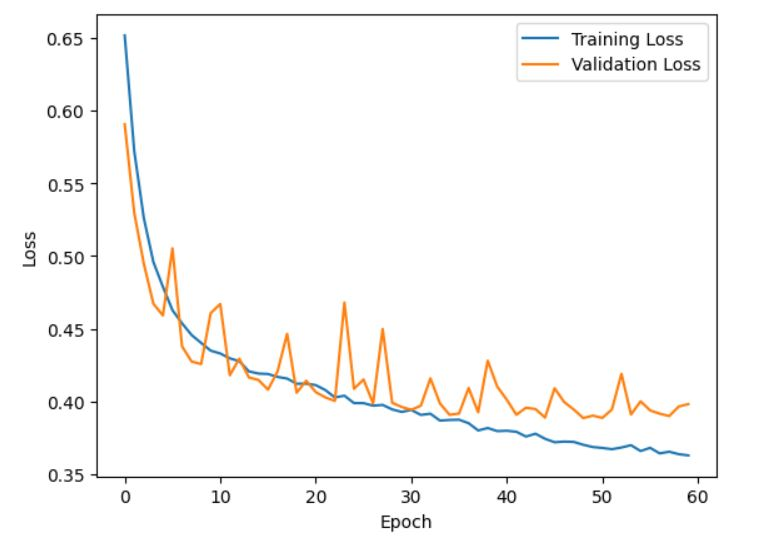
\includegraphics[width=0.75\textwidth]{resim.JPG}
    \caption{Buraya açıklama yazın}
    \label{fig:my_pic}
\end{figure}
% Figure aşağıda comment içindeki kısımdaki gibi eklenir.
\begin{comment}
\begin{figure}[ht!]
    \centering
    \includegraphics[width=0.75\textwidth]{mypicturehere.png}
    \caption{Buraya açıklama yazın}
    \label{fig:my_pic}
\end{figure}
\end{comment}



\subsection{(10 Puan)} \textbf{SEED=öğrenci numaranız set ettikten sonra altıncı haftada ödev olarak verdiğim gibi earlystopping'deki en iyi modeli kullanarak, Prensesi İyileştir test setinden accuracy, F1, precision ve recall değerlerini hesaplayan kodu yazın ve sonucu da aşağı yapıştırın. \%80'den fazla başarı bekliyorum test setinden. Daha düşükse başarı oranınız, nerede hata yaptığınızı bulmaya çalışın. \%90'dan fazla başarı almak mümkün (ben denedim).

}

\begin{python}
checkpoint = torch.load('/content/drive/MyDrive/dataset/checkpoint.pt')
model_2 = MLP(input_dim, output_neuron)
model_2.load_state_dict(checkpoint)
model_2.to(device)

\end{python}

\begin{python}

 validation_score = validation_loss
        if best_validation_loss is None:
          patience_counter = 0
          best_validation_loss = validation_score
          torch.save(model.state_dict(), "checkpoint.pt")
        elif best_validation_loss < validation_score:
          patience_counter += 1
          print("Earlystopping Patience Counter", patience_counter)
          if patience_counter == patience:
              break
        else:
          best_validation_loss = validation_score
          torch.save(model.state_dict(), "checkpoint.pt")
          patience_counter = 0
\end{python}

\begin{python}
evaluate_metrics(model_2, criterion, test_loader)
\end{python}

 Test Accuracy: 0.9236,Prec Accuracy: 0.9237,F1 score: 0.9236,Recall score: 0.9236

\subsection{(5 Puan)} \textbf{Tüm kodların CPU'da çalışması ne kadar sürüyor hesaplayın. Sonra to device yöntemini kullanarak modeli ve verileri GPU'ya atıp kodu bir de böyle çalıştırın ve ne kadar sürdüğünü hesaplayın. Süreleri aşağıdaki tabloya koyun. GPU için Google Colab ya da Kaggle'ı kullanabilirsiniz, iki ortam da her hafta saatlerce GPU hakkı veriyor.}

\begin{table}[ht!]
    \centering
    \caption{PyTorch kütüphanesinin device sınıfı kullanılarak çalışma zamanı ölçülmüştür. }
    \begin{tabular}{c|c}
        Ortam & Süre (saniye) \\\hline
        CPU & 0:00:08.260194  \\
        GPU & 0:00:17.042746\\
    \end{tabular}
    \label{tab:my_table}
\end{table}


\subsection{(3 Puan)} \textbf{Modelin eğitim setine overfit etmesi için elinizden geldiği kadar kodu gereken şekilde değiştirin, validasyon loss'unun açıkça yükselmeye başladığı, training ve validation loss'ları içeren figürü aşağı koyun ve overfit için yaptığınız değişiklikleri aşağı yazın. Overfit, tam bir çanak gibi olmalı ve yükselmeli. Ona göre parametrelerle oynayın.}

 \textbf{Cevap = } Overfit için epoch değerlerinde ve earlystopping de en iyi sonucu oluşturmak için patience üzerinde de oynamalar yapılmıştır. Gerekli denemeler sonucu en iyi sonuç oluşturulmaya çalışılmıştır. Regülarizasyon çalışmları yapılmaya çalışılmıştır.Ortaya aşağıdaki görsel çıkmıştır.

\begin{figure}[ht!]
    \centering
    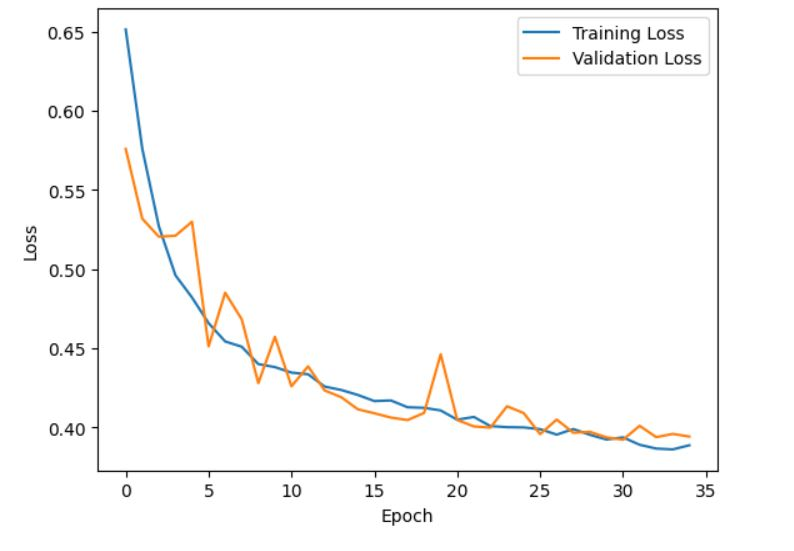
\includegraphics[width=0.75\textwidth]{alinti.JPG}
    \caption{Overfit çalışmaları sonucu}
    \label{fig:my_pic}
\end{figure}

\subsection{(2 Puan)} \textbf{Beşinci soruya ait tüm kodların ve cevapların olduğu jupyter notebook'un Github linkini aşağıdaki url'e koyun.}

\url{https://github.com/oznurkan/Project_artificial_neural_network_2}

\section{(Toplam 10 Puan)} \textbf{Bir önceki sorudaki Prensesi İyileştir problemindeki yapay sinir ağınıza seçtiğiniz herhangi iki farklı regülarizasyon yöntemi ekleyin ve aşağıdaki soruları cevaplayın.} 

\subsection{(2 puan)} \textbf{Kodlarda regülarizasyon eklediğiniz kısımları aşağı koyun:} 

\begin{python}
kod_buraya = None
if kod_buraya:
    devam_ise_buraya = 0

print(devam_ise_buraya)
\end{python}

\subsection{(2 puan)} \textbf{Test setinden yeni accuracy, F1, precision ve recall değerlerini hesaplayıp aşağı koyun:}

Sonuçlar buraya.

\subsection{(5 puan)} \textbf{Regülarizasyon yöntemi seçimlerinizin sebeplerini ve sonuçlara etkisini yorumlayın:}

Yorumlar buraya.

\subsection{(1 puan)} \textbf{Sonucun github linkini  aşağıya koyun:}

\url{www.benimgithublinkim2.com}

\end{document}